\chapter{Metodologia}
\label{chap:metod}
Nesta capitulo será descrito os procedimento, com os materias e métodos, para a realização do estudo do esuto da arte de ROVs que realizam ações de forma autonoma.

O metodo usado para alcançar o objetivo deste material foi o método BILI que consiste em executar uma busca otmizada de publicações sobre temas especificos.

\section{Metódo BilI}

O Método BiLi usa bibliotecas que estão presente na liguagem de progamação R,  a plataforma Mendely e a ferramenta cmpatools. A Figura \ref{fig:metodo_bili} demostra um fluxograma que representa a aplicação do Metodo Bili.  ANas próximas sessões serão apresentadas  cada etapa deste método.

%---------------picture------------------------------------
\begin{figure}
    \centering
   
    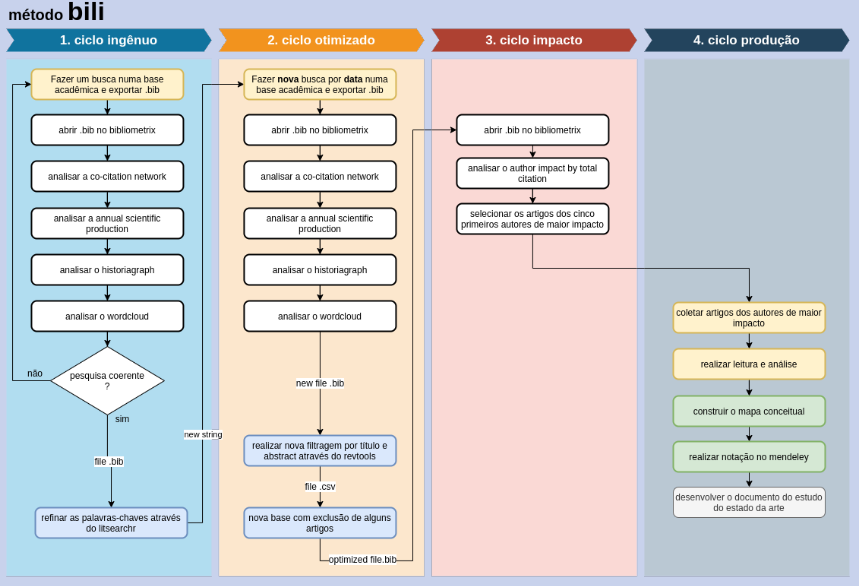
\includegraphics[width=\textwidth]{metodo_bili.png}
    \caption{Método Bili}
    \label{fig:metodo_bili}
\end{figure}
%----------------------------------------------------------